% CORA poster, ARC Prize Research Summit, 23 October 2026.
% Every number is indexed in records/CORA_SUMMIT_POSTER_EVIDENCE_20261012.md.
% Every image is in figures/ and is drawn from sealed outputs by
% scripts/summit_figures.py; diagrams are TikZ drawings of the real pipeline.
\documentclass[25pt, a0paper, portrait, margin=0mm, innermargin=14mm,
  blockverticalspace=12mm, colspace=14mm, subcolspace=8mm]{tikzposter}
\usepackage[scaled]{helvet}
\renewcommand{\familydefault}{\sfdefault}
\usepackage{graphicx}
\usepackage{booktabs}
\usepackage{array}
\usetikzlibrary{positioning, arrows.meta, shapes.misc, fit, calc}

\definecolor{ink}{HTML}{0B0B0B}
\definecolor{ink2}{HTML}{52514E}
\definecolor{muted}{HTML}{898781}
\definecolor{accent}{HTML}{2A78D6}
\definecolor{warm}{HTML}{EB6834}
\definecolor{neutral}{HTML}{F0EFEC}
\definecolor{critical}{HTML}{D03B3B}
\definecolor{paper}{HTML}{FCFCFB}

\usetheme{Simple}
\tikzposterlatexaffectionproofoff
\makeatletter
\settitle{\centering\vbox{\color{titlefgcolor}{\bfseries\Huge \@title\par}\vspace*{0.7em}{\huge \@author\par}\vspace*{0.5em}{\LARGE \@institute}}}
\makeatother
\colorlet{backgroundcolor}{paper}
\colorlet{framecolor}{paper}
\colorlet{titlefgcolor}{ink}
\colorlet{titlebgcolor}{paper}
\colorlet{blocktitlebgcolor}{paper}
\colorlet{blocktitlefgcolor}{accent}
\colorlet{blockbodybgcolor}{paper}
\colorlet{blockbodyfgcolor}{ink}
\colorlet{innerblocktitlebgcolor}{neutral}
\colorlet{innerblocktitlefgcolor}{ink}
\colorlet{innerblockbodybgcolor}{neutral}
\colorlet{innerblockbodyfgcolor}{ink}

\title{\parbox{0.92\linewidth}{\centering When Search Is Not Enough: Diagnosing Failure Before\\
  Constructing Verified Reasoning Capabilities}}
\author{Chimdi Walter Ndubuisi \quad (University of Missouri)}
\institute{CORA on ARC-AGI-2 \;$\cdot$\; development results \;$\cdot$\; ARC Prize Research Summit, 23 October 2026}

\tikzset{
  stage/.style={rounded corners=6pt, draw=accent, line width=1.8pt, fill=white, align=center,
                font=\normalsize, minimum height=2.8cm, text width=19cm, inner sep=10pt},
  choice/.style={rounded corners=6pt, draw=ink2, line width=1.4pt, fill=neutral, align=center,
                 font=\small, minimum height=3.0cm, text width=4.9cm, inner sep=6pt},
  planned/.style={choice, dashed, fill=white},
  flow/.style={-{Latex[length=6mm,width=4mm]}, line width=2pt, draw=ink2},
}

\begin{document}
\maketitle[width=0.96\linewidth]

\begin{columns}
% ======================================================================
\column{0.333}
\block{The question}{
  \centering\large\textbf{How can a reasoning system know when its existing way of solving problems is
  inadequate, and acquire a better one without compromising the evidence used to judge it?}\par
  \vspace{0.6em}\normalsize\raggedright
  A failure to solve is ambiguous. It can mean:
  \begin{itemize}
    \item \textbf{search}: a program exists in the bounded language, but search missed it;
    \item \textbf{representation}: the right object view was screened out before induction;
    \item \textbf{expressivity}: the bounded language holds no solution (needs a complete check);
    \item \textbf{evidence}: the demonstrations support incompatible rules;
    \item \textbf{verification}: a valid candidate is rejected or not reproduced when examples change.
  \end{itemize}
  These call for different responses: search longer, change the view, construct an executable
  extension, or abstain.\par
  \vspace{0.4em}\centering\textit{Self-modifying executable knowledge,\\ with non-self-modifying standards of evidence.}
}

\block{The CORA loop}{
  \begin{tikzfigure}
  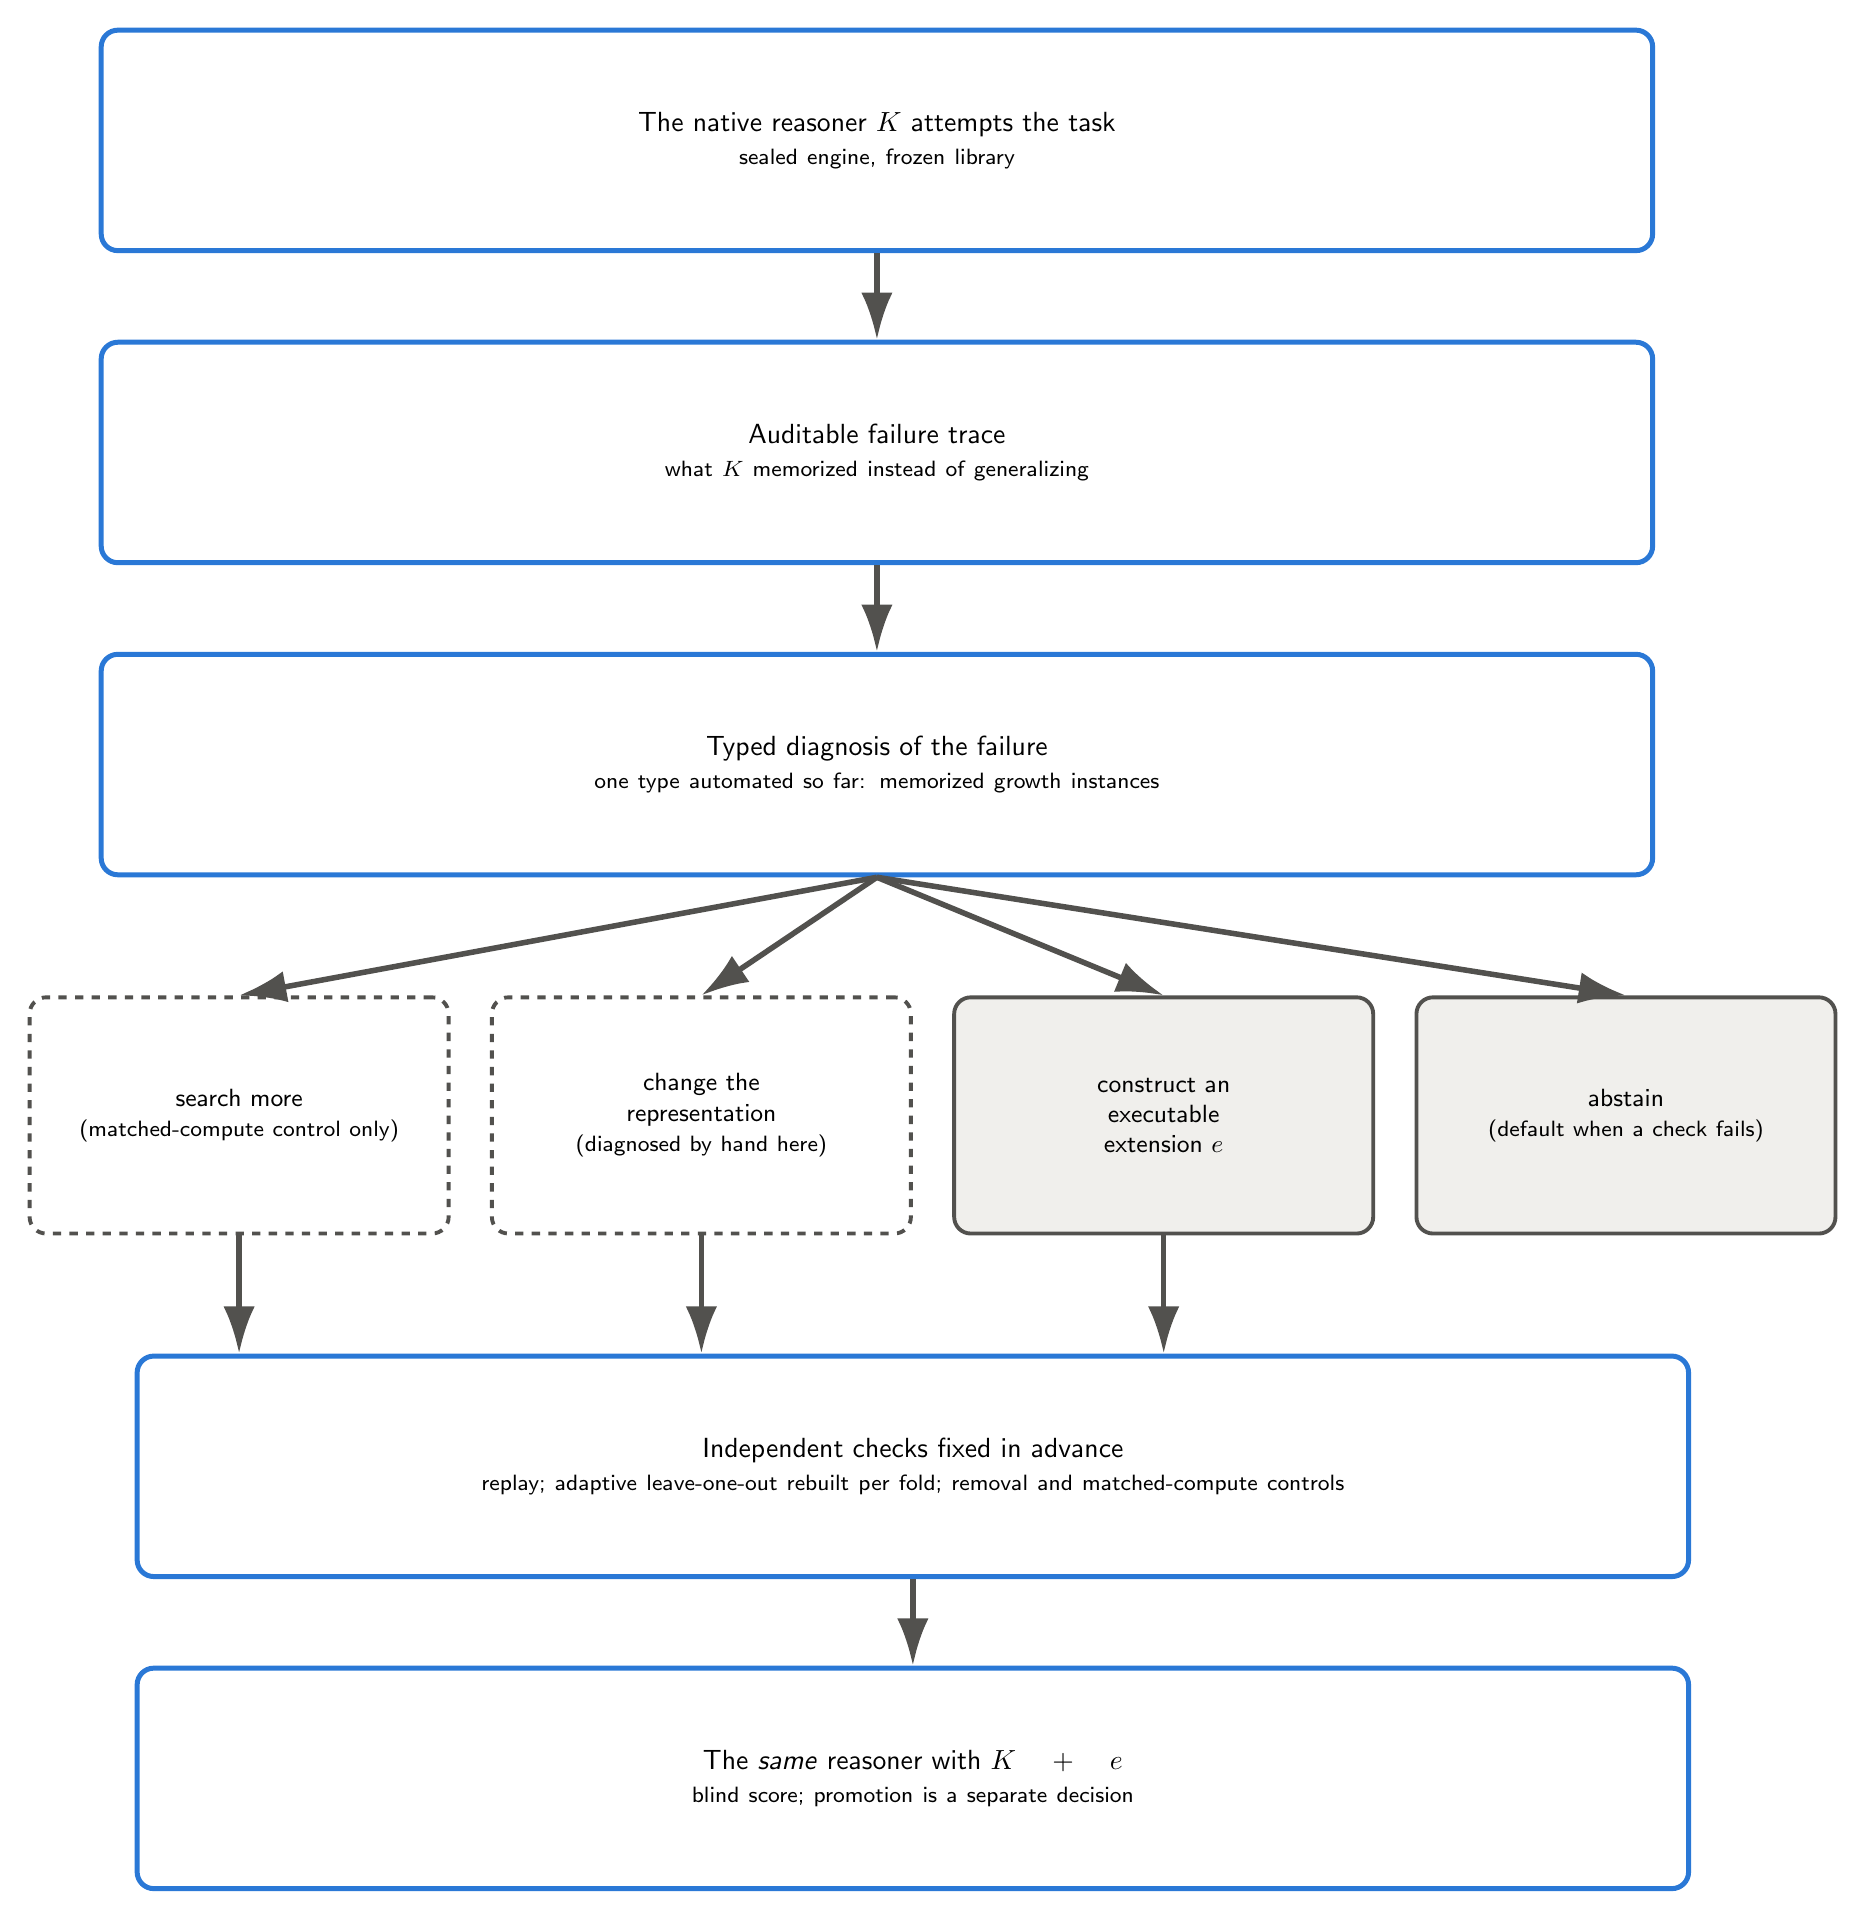
\begin{tikzpicture}[node distance=1.1cm]
    \node[stage] (k) {The native reasoner $K$ attempts the task\\ \footnotesize sealed engine, frozen library};
    \node[stage, below=of k] (t) {Auditable failure trace\\ \footnotesize what $K$ memorized instead of generalizing};
    \node[stage, below=of t] (d) {Typed diagnosis of the failure\\ \footnotesize one type automated so far: memorized growth instances};
    \node[planned, below=1.5cm of d, xshift=-8.1cm] (c1) {search more\\ \footnotesize (matched-compute control only)};
    \node[planned, right=0.5cm of c1] (c2) {change the\\ representation\\ \footnotesize (diagnosed by hand here)};
    \node[choice, right=0.5cm of c2] (c3) {construct an\\ executable\\ extension $e$};
    \node[choice, right=0.5cm of c3] (c4) {abstain\\ \footnotesize (default when a check fails)};
    \node[stage, below=1.5cm of c2.south east] (v) {Independent checks fixed in advance\\ \footnotesize replay; adaptive leave-one-out rebuilt per fold; removal and matched-compute controls};
    \node[stage, below=of v] (r) {The \emph{same} reasoner with $K+e$\\ \footnotesize blind score; promotion is a separate decision};
    \draw[flow] (k) -- (t);
    \draw[flow] (t) -- (d);
    \foreach \c in {c1, c2, c3, c4} \draw[flow] (d.south) -- (\c.north);
    \foreach \c in {c1, c2, c3} \draw[flow] (\c.south) -- (v.north -| \c.south);
    \draw[flow] (v) -- (r);
  \end{tikzpicture}
  \end{tikzfigure}
  \small Solid boxes are implemented and measured; dashed ones are specified but not automated.
  Four claims are kept apart and never inferred from each other: \textbf{C1} the extension installs and
  runs; \textbf{C2} $K+e$ beats $K$ and matched removal and compute controls; \textbf{C3} the real
  failure trace adds value over demonstrations-only and shuffled-failure construction; \textbf{C4} a
  retained capability helps later unseen tasks.
}

\block{Evidence ledger}{
  \footnotesize
  \begin{tabular}{@{}>{\raggedright}p{0.74\linewidth}l@{}}
    \toprule
    synthetic v1.9 prospective (27/30 vs 12/30) & 2885a04\\
    real reach v1 measurement, verified (4/60 installed, 0/14 LOO) & bb11f95\\
    adaptive-LOO diagnosis record & c2b8cd4\\
    segmentation-admission probes & 955542c, 82251a4\\
    representation-eligibility addendum, P2 proposal (not authorized) & a719383\\
    synthetic negative controls; static exposure & 70d3ed9, 3ba75e5\\
    pilot v2 frozen, not run (N = 120) & c1906ee\\
    \bottomrule
  \end{tabular}\par
  \vspace{0.3em}Index: \texttt{records/CORA\_SUMMIT\_POSTER\_EVIDENCE\_20261012.md}
}

\block{Take-home}{
  \begin{enumerate}
    \item A failed solve is not one thing. On real ARC development tasks the blocker we traced was
      \textbf{representation admission} (a search-layer defect in the native engine), not a missing capability.
    \item The obvious repair, forcing the right view, was \textbf{harmful} on synthetic controls. Negative
      controls come before any repair is run.
    \item Constructed extensions now reach the native engine (0/60 to 4/60 installed; one accepted and
      used), but \textbf{none survives adaptive leave-one-out}; no new ARC solve is claimed.
  \end{enumerate}
}

% ======================================================================
\column{0.333}
\block{What has been measured}{
  \begin{tikzfigure}
    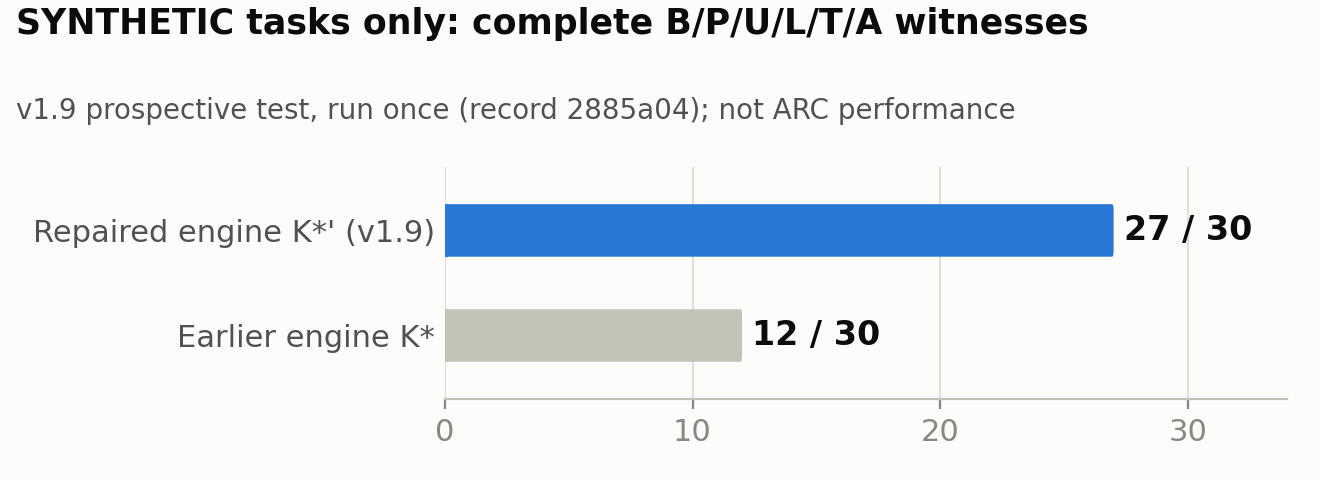
\includegraphics[width=0.98\linewidth]{figures/fig_synthetic_v19.png}
  \end{tikzfigure}
  \small Synthetic, frozen, run once: the claim is LEVEL 2 for that synthetic domain only. The repaired
  engine also accepted every deliberately wrong installed extension it was given (5/5 and 28/28), so
  safety must come from task-time verification, not from engine acceptance.
  \begin{tikzfigure}
    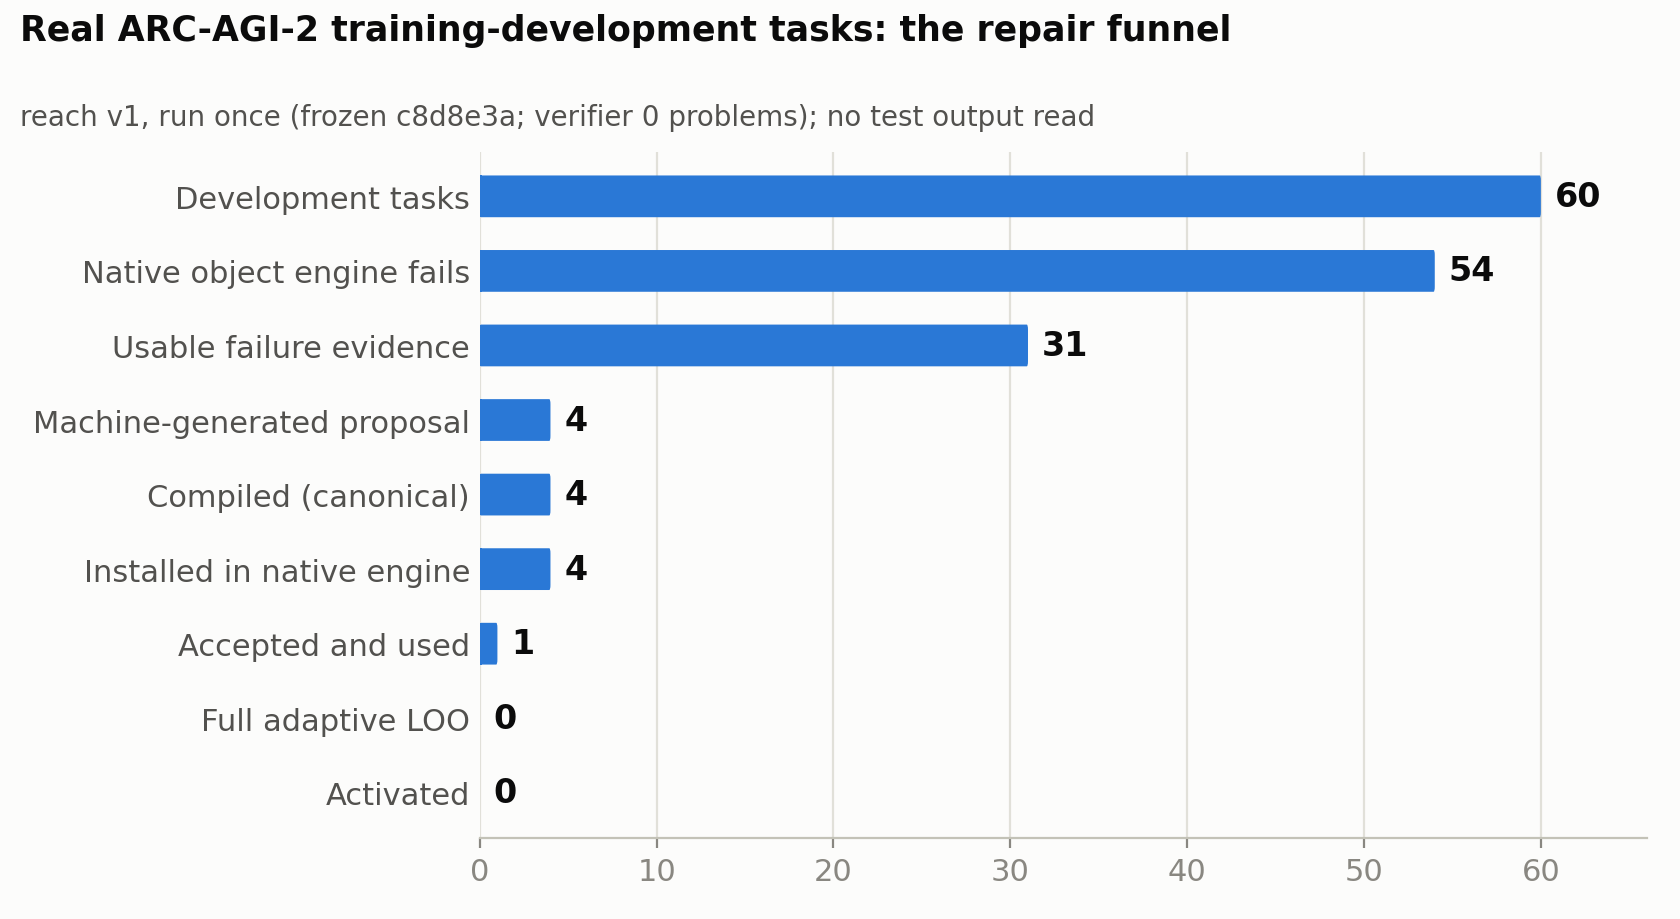
\includegraphics[width=0.98\linewidth]{figures/fig_funnel_reach_v1.png}
  \end{tikzfigure}
  \small Real ARC-AGI-2 \emph{training-development} tasks, no test output read. Installation rose from 0/60
  to 4/60; one repair was accepted and used with all demonstrations; \textbf{none survived adaptive
  leave-one-out (0 of 14 folds); 0 activations}. No new ARC solve is claimed; the certified training
  score stays 185/1{,}000. A preserved negative: an earlier failure-association selector did not beat
  demonstrations alone (0.585 vs 0.591, 288 synthetic groups).
}

\block{A forensic counterexample to ``just search harder''}{
  \begin{tikzfigure}
    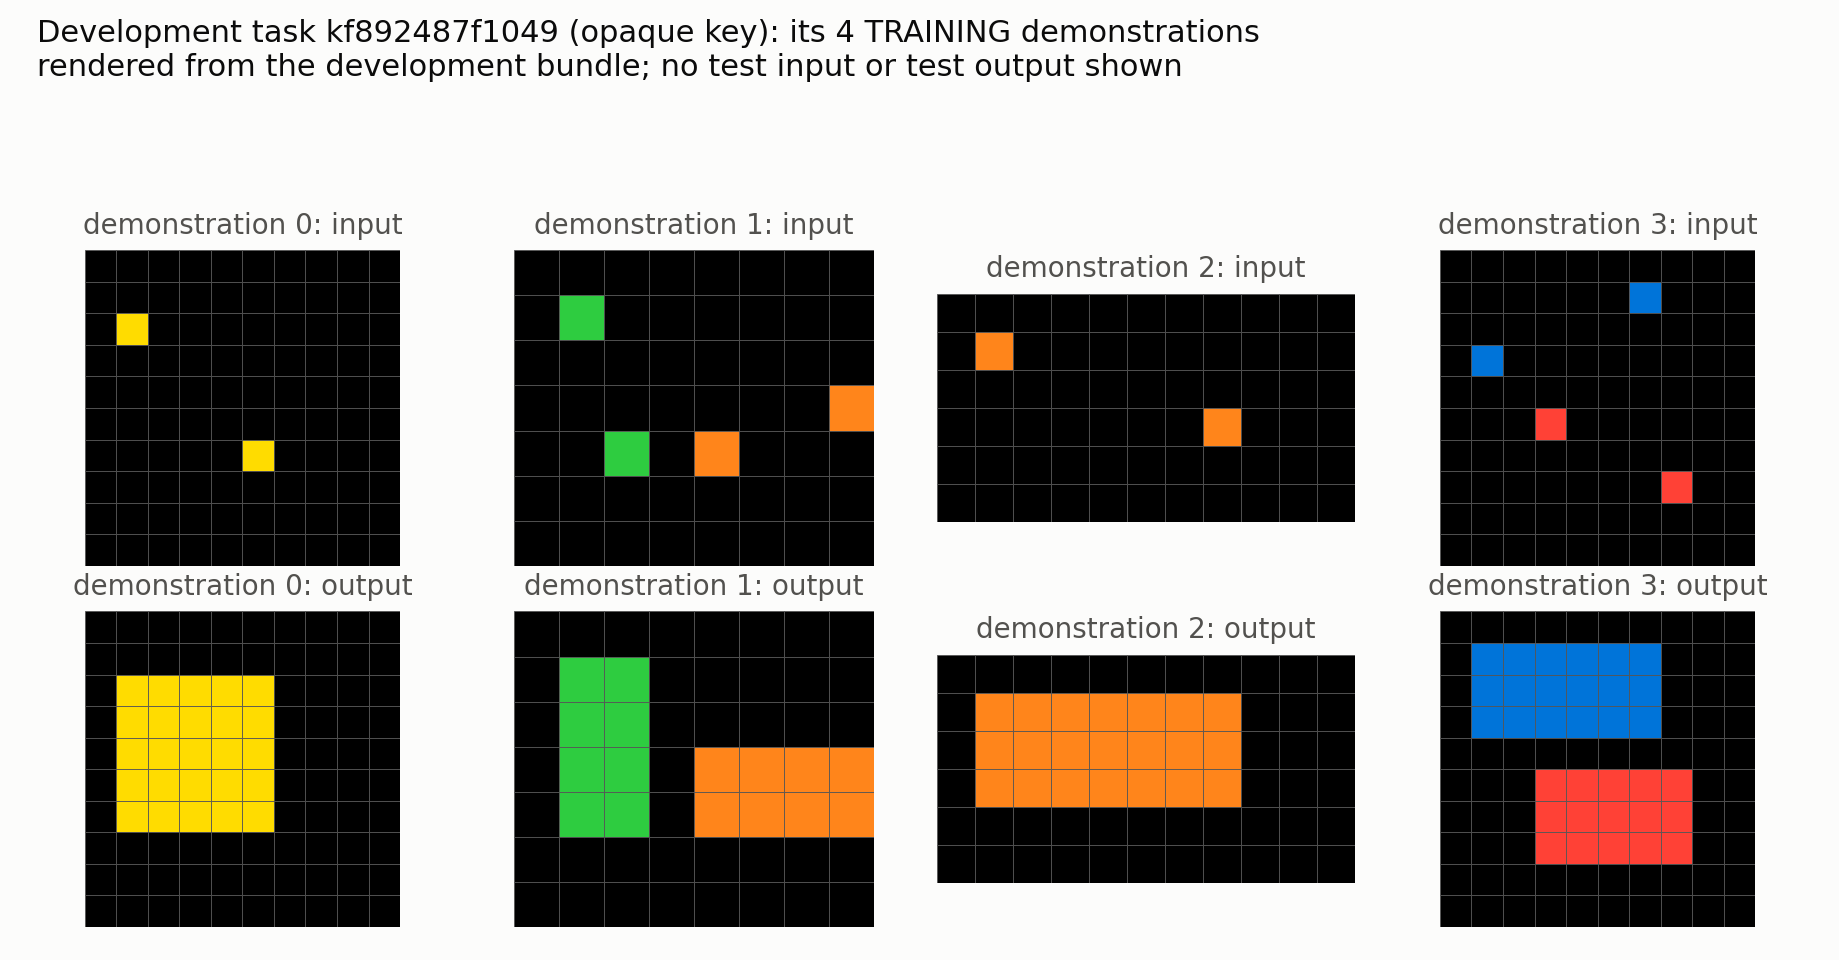
\includegraphics[width=0.98\linewidth]{figures/fig_kf89_training_demonstrations.png}
  \end{tikzfigure}
  \small CORA built a \texttt{bbox\_fill} growth relation from the engine's own memorized failures; with
  all four demonstrations the unchanged engine accepted the one-rule program $G$ and used it. Rebuilding
  without one demonstration fails: the engine's own leave-one-out must re-induce from two.
  \begin{tikzfigure}
    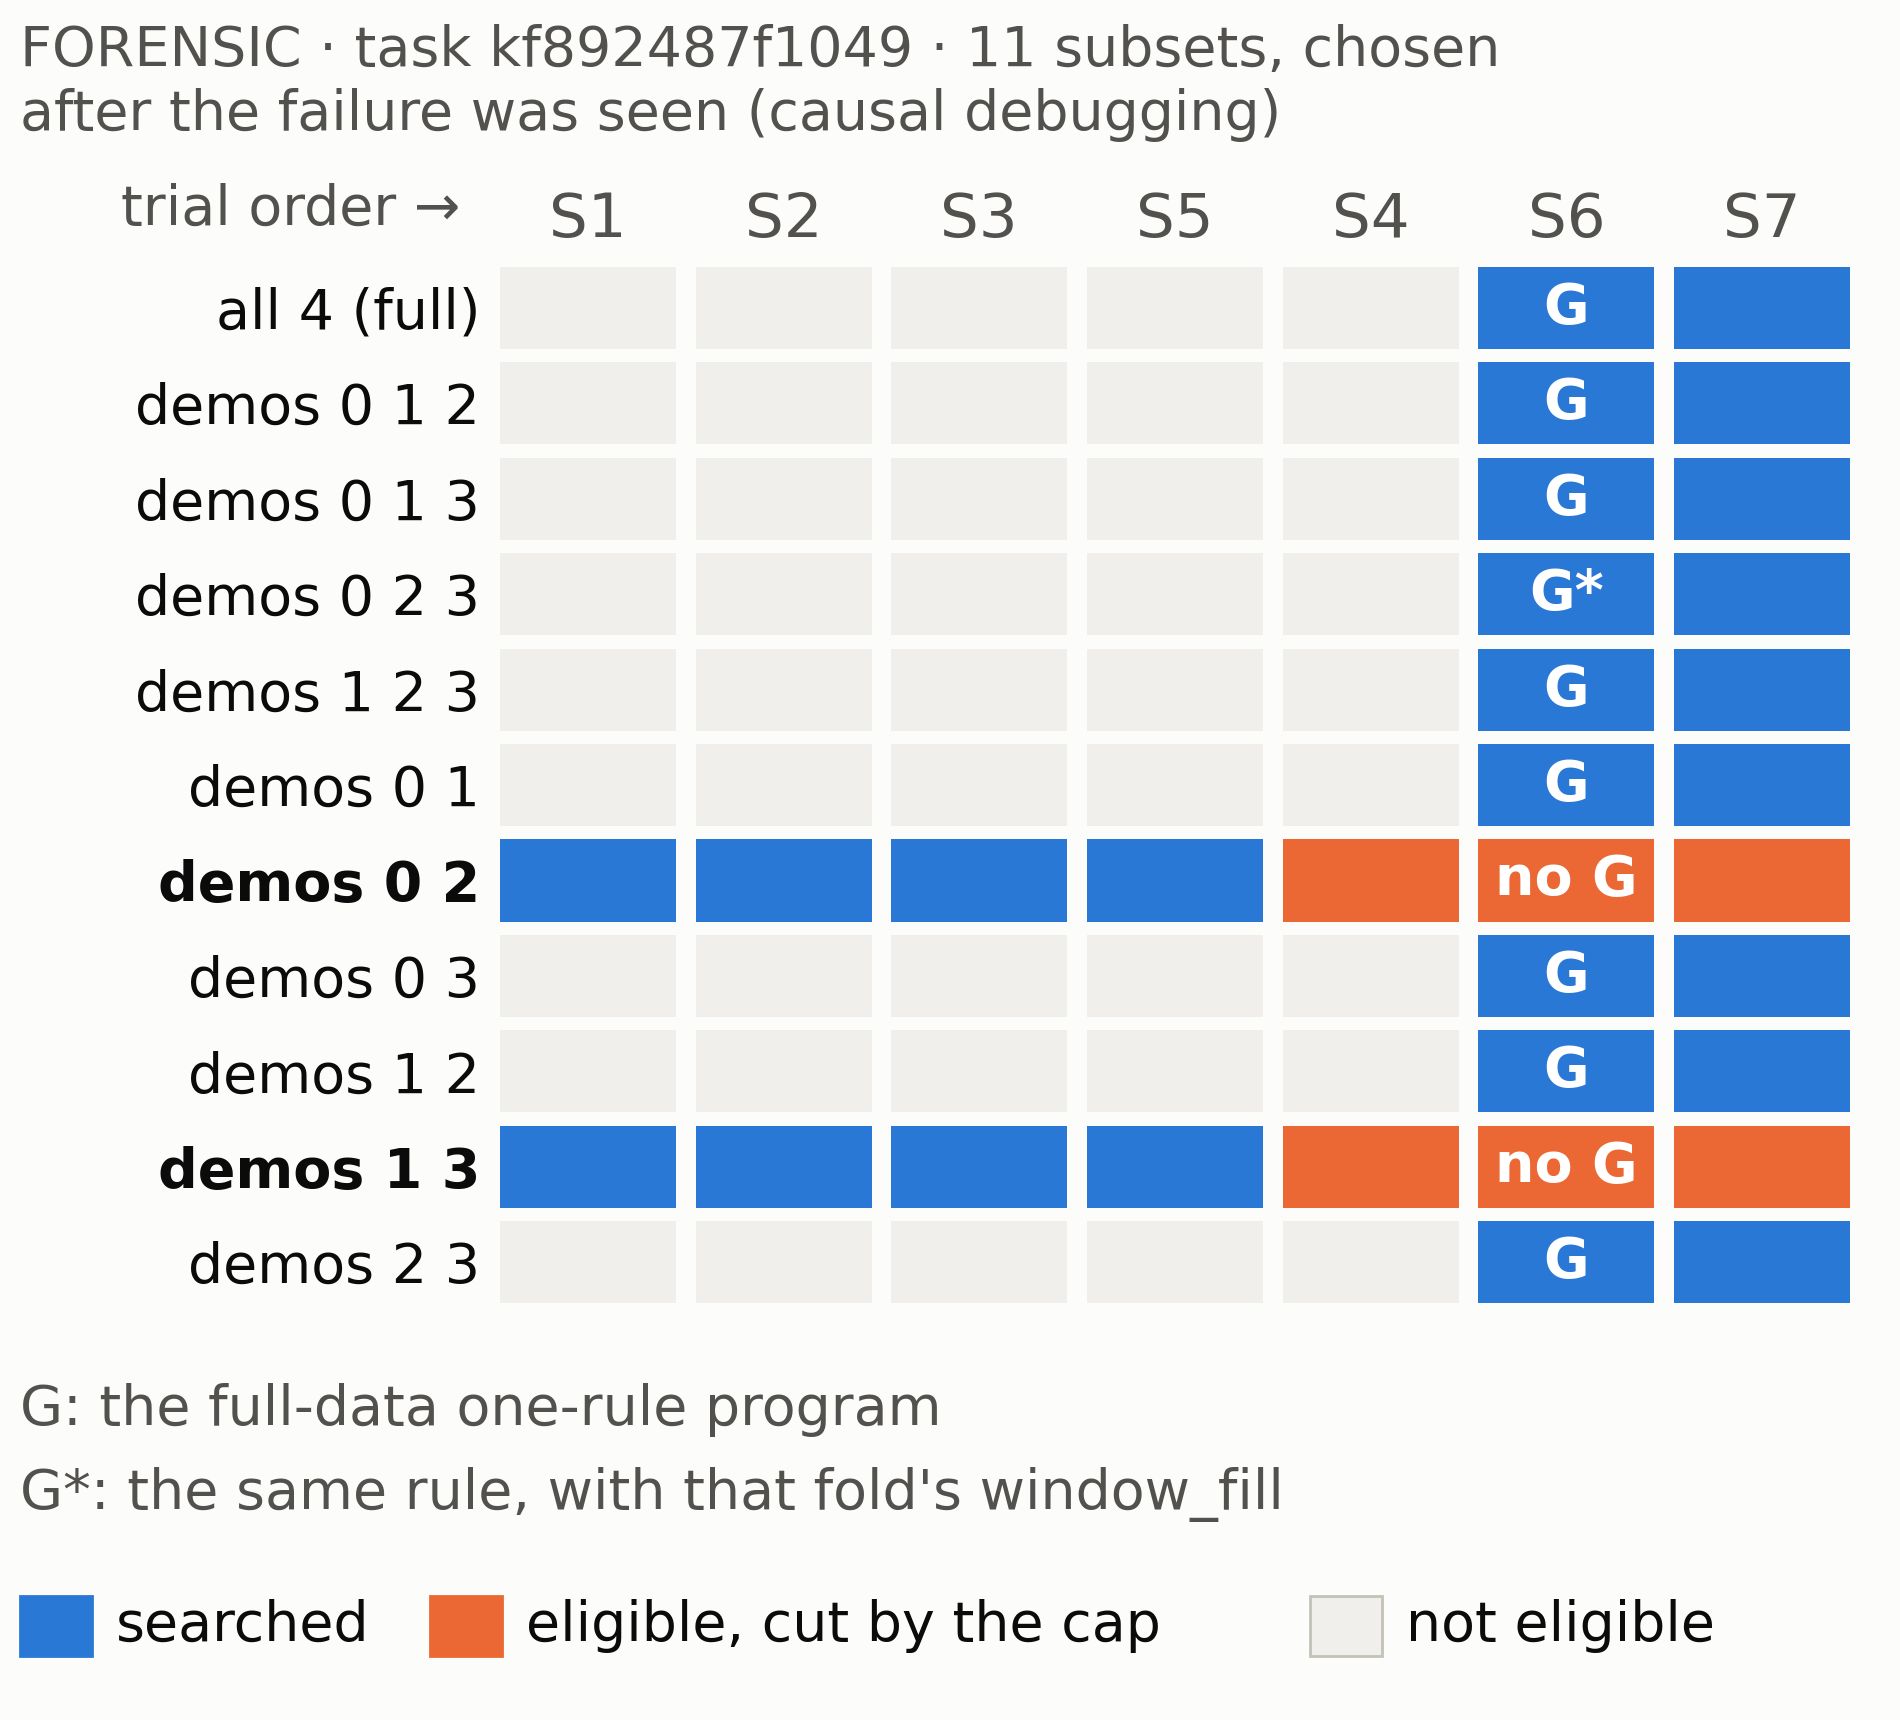
\includegraphics[width=0.98\linewidth]{figures/fig_kf89_variant_admission.png}
  \end{tikzfigure}
  \small \textbf{The mechanism.} The engine searches at most 4 eligible segmentation variants in a fixed
  order. In the fine variants the demonstrations have object counts $(2\!\to\!1),(4\!\to\!2),(2\!\to\!1),(4\!\to\!2)$:
  no common count relation, so they are ineligible, except on the pairs $\{0,2\}$ and $\{1,3\}$, where a
  constant difference makes them eligible and they fill the cap. The correct view (S6) stays eligible and
  is strictly coarser, but is never searched; $G$ is valid on those pairs yet never generated. The
  eligibility rule behaves as designed (removing demonstrations never removes an eligible view); the cap
  defeats the engine's own rule that a coarser view is still tried so that folds converge.
  Development only; the pairs were examined after the failure was seen.
}

% ======================================================================
\column{0.333}
\block{Negative controls before any repair}{
  \begin{tikzfigure}
    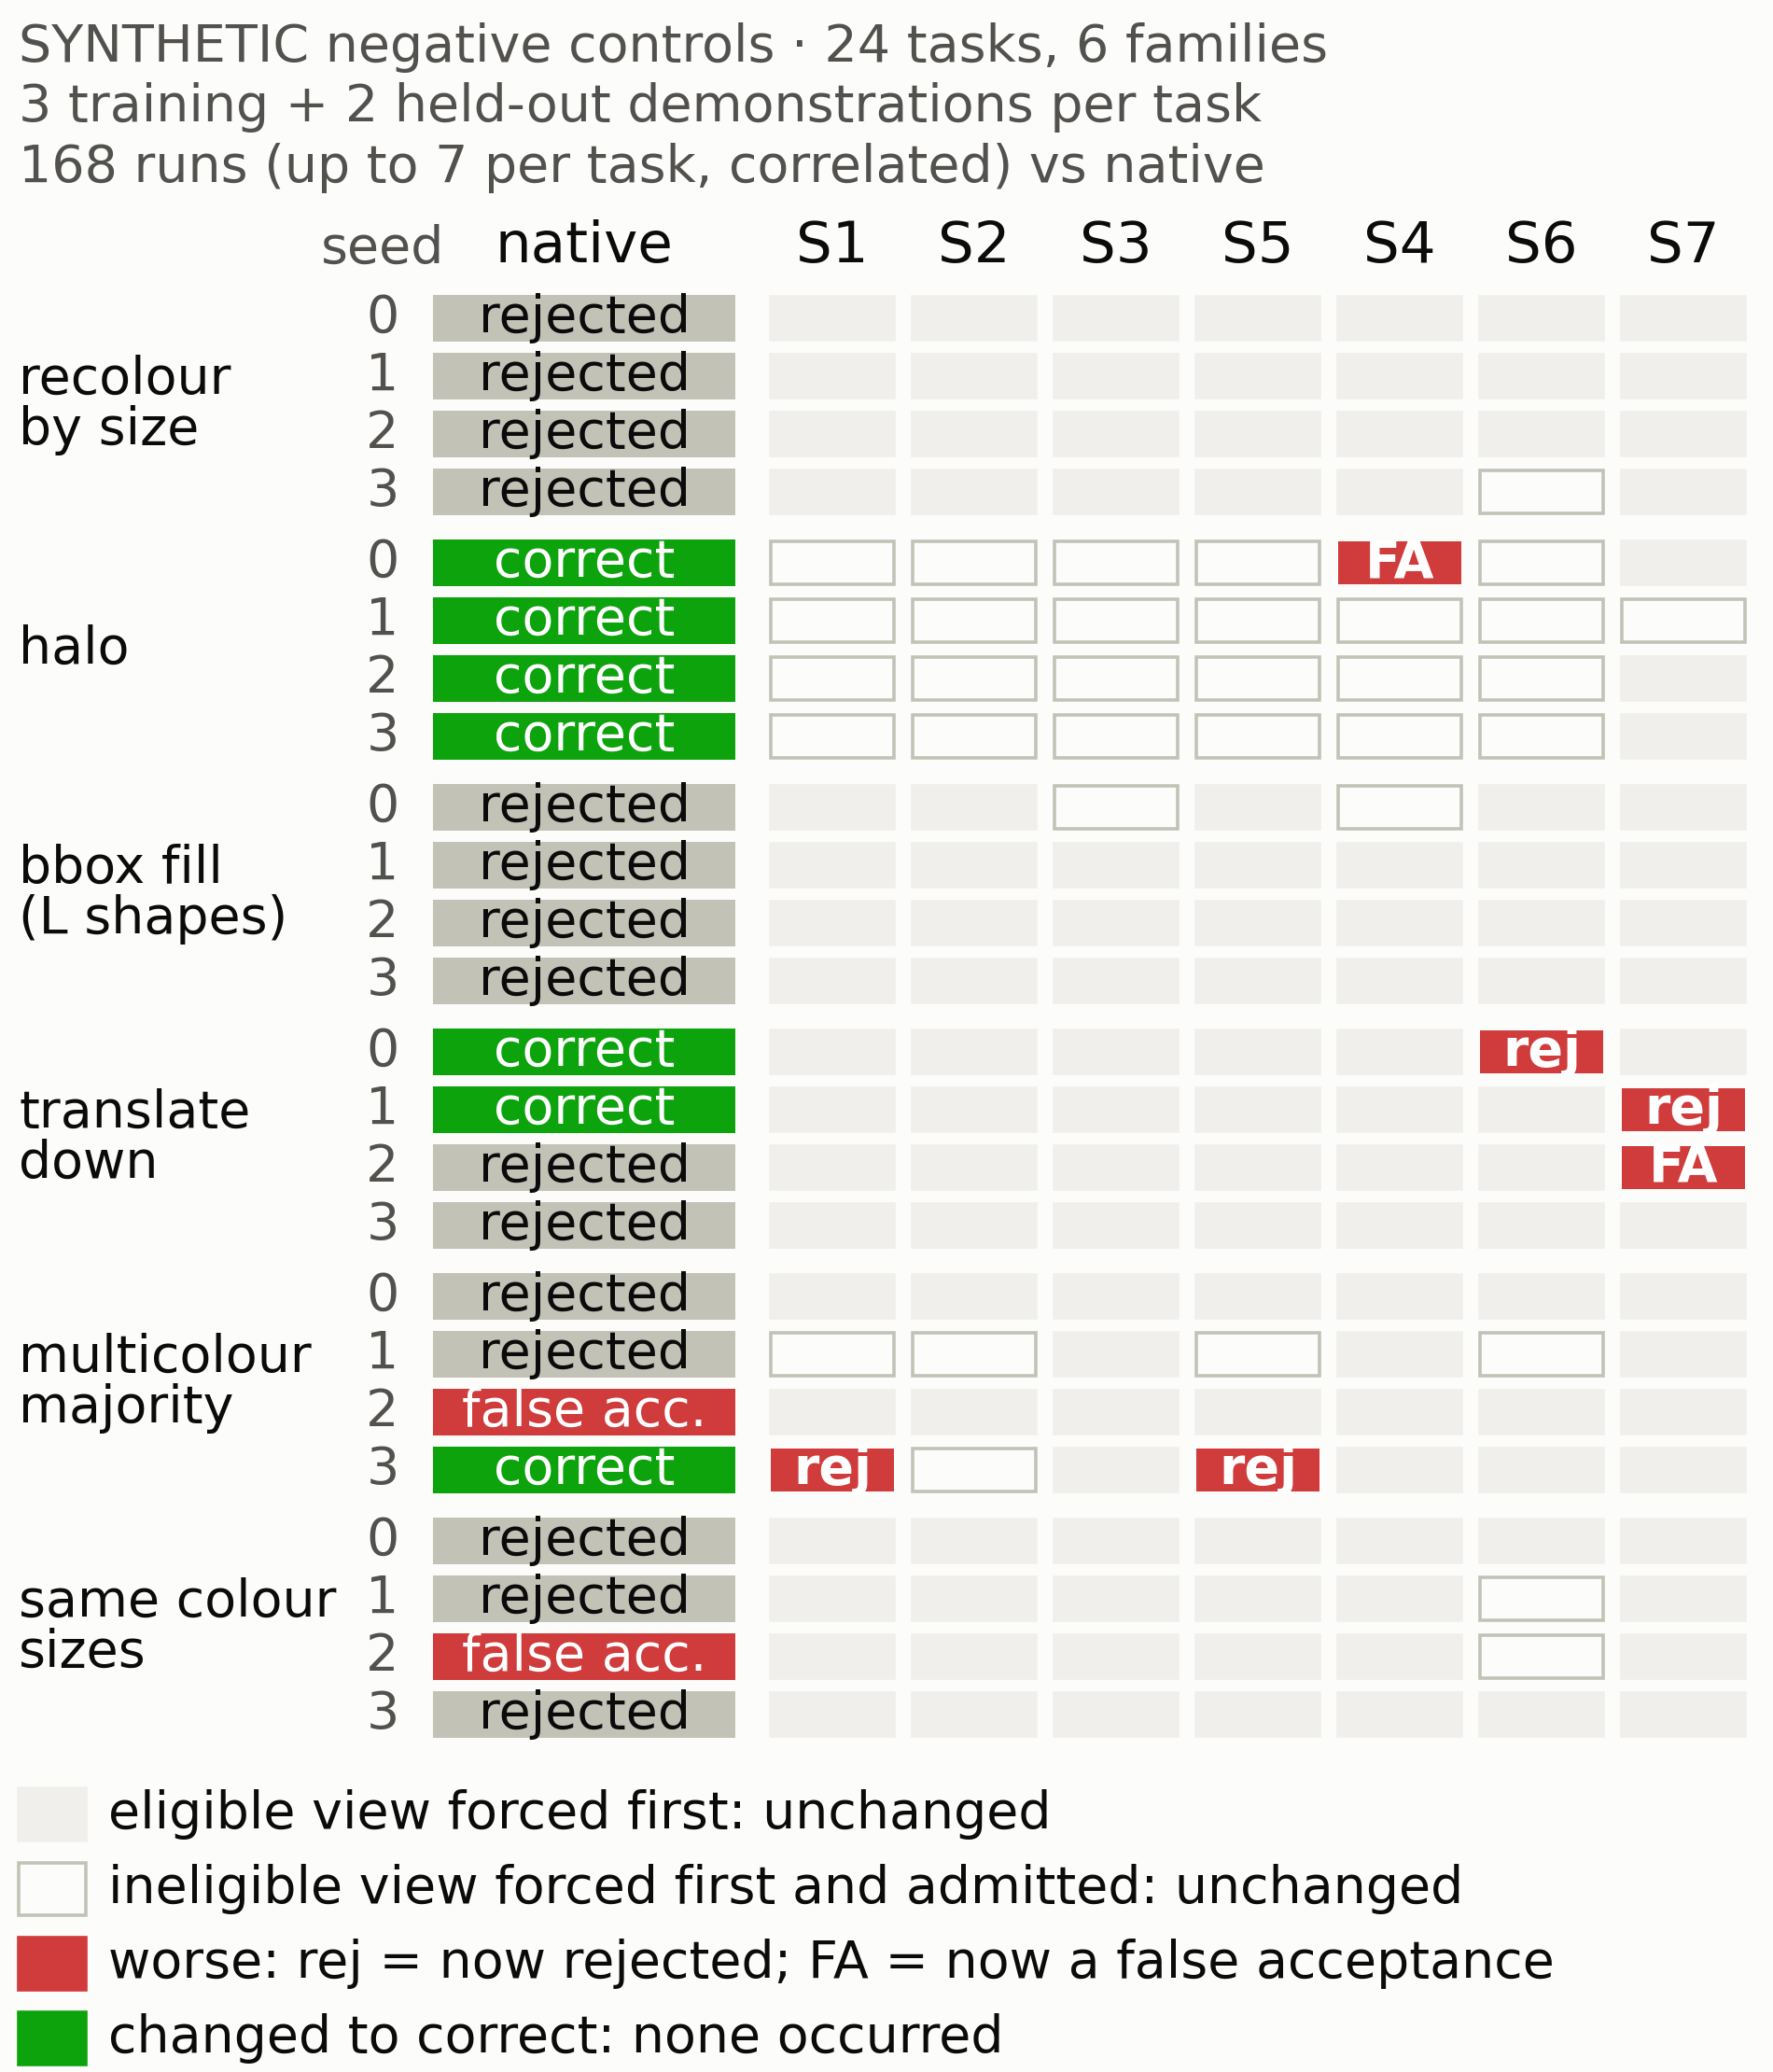
\includegraphics[width=0.98\linewidth]{figures/fig_negative_controls.png}
  \end{tikzfigure}
  \small A fix that makes the known task pass proves nothing by itself, so the candidate repairs were
  first tried on synthetic tasks with known rules and held-out demonstrations. Forcing one segmentation
  view to be searched first, whether it was eligible or not, produced \textbf{no gains and six harmful
  changes in 168 paired runs}: correct native answers became rejections or false acceptances. We
  therefore did not run the variant-first repair we had built. Letting the engine reach every cut view
  would change the search on 73 of 96 synthetic subsets, so that is not narrow either.
}

\block{A domain-portable protocol, not a domain-free oracle}{
  \begin{tikzfigure}
  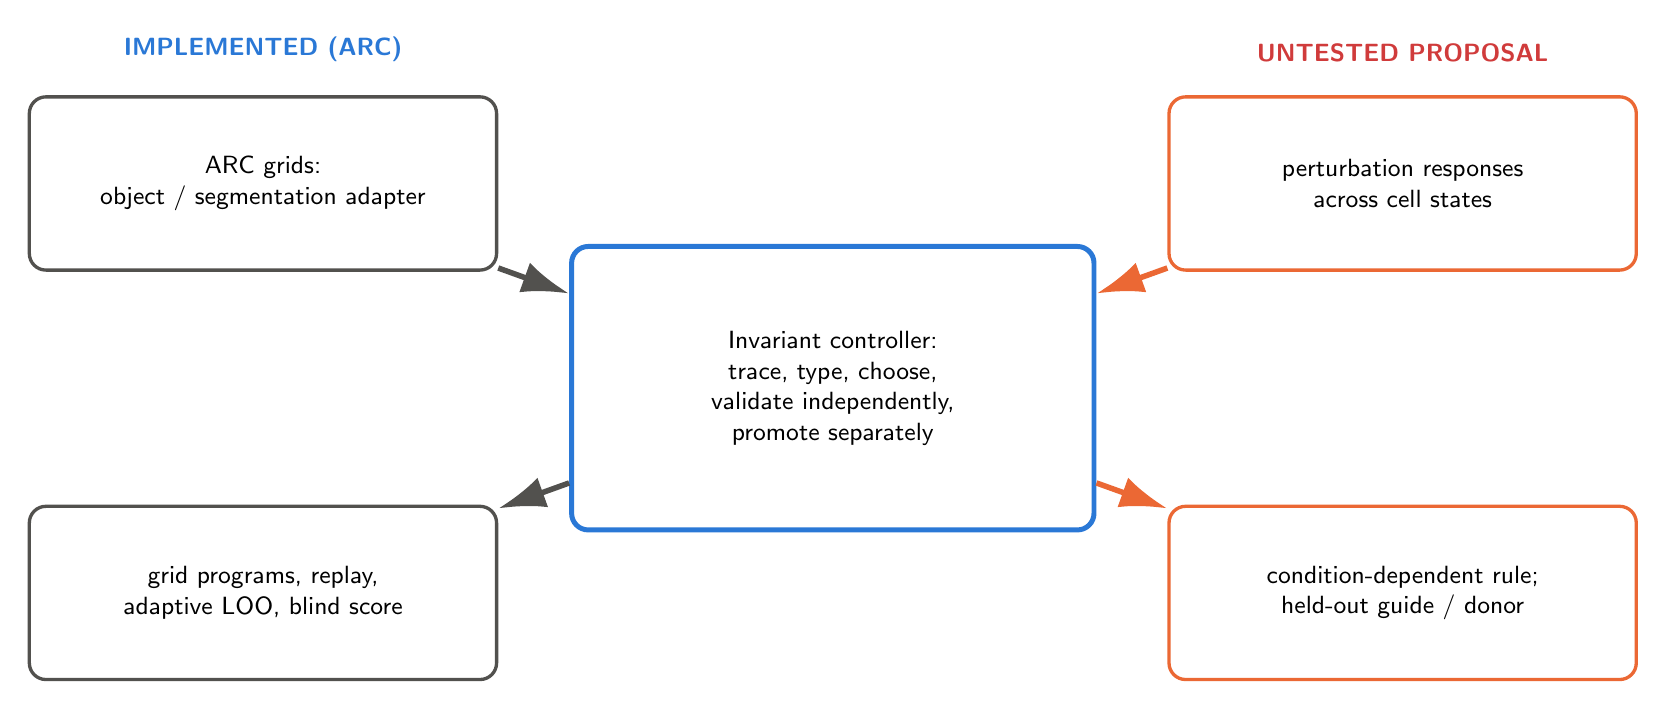
\begin{tikzpicture}[lane/.style={rounded corners=6pt, draw=ink2, line width=1.2pt, fill=white,
        align=center, font=\small, text width=5.7cm, minimum height=2.2cm},
      core/.style={rounded corners=6pt, draw=accent, line width=1.8pt, fill=white, align=center,
        font=\small, text width=6.4cm, minimum height=3.6cm}]
    \node[core] (ctl) {Invariant controller:\\ trace, type, choose,\\ validate independently,\\ promote separately};
    \node[lane, left=0.9cm of ctl, yshift=2.6cm] (a1) {ARC grids:\\ object / segmentation adapter};
    \node[lane, left=0.9cm of ctl, yshift=-2.6cm] (a2) {grid programs, replay,\\ adaptive LOO, blind score};
    \node[lane, right=0.9cm of ctl, yshift=2.6cm, draw=warm] (b1) {perturbation responses\\ across cell states};
    \node[lane, right=0.9cm of ctl, yshift=-2.6cm, draw=warm] (b2) {condition-dependent rule;\\ held-out guide / donor};
    \draw[flow] (a1) -- (ctl); \draw[flow] (ctl) -- (a2);
    \draw[flow, draw=warm] (b1) -- (ctl); \draw[flow, draw=warm] (ctl) -- (b2);
    \node[above=0.3cm of a1, font=\small\bfseries, text=accent] {IMPLEMENTED (ARC)};
    \node[above=0.3cm of b1, font=\small\bfseries, text=critical] {UNTESTED PROPOSAL};
  \end{tikzpicture}
  \end{tikzfigure}
  \small The control logic is meant to transfer; observations, program semantics, priors and
  validators do not. The biological lane has \textbf{no data and no results}: it would need
  leave-one-guide and leave-one-donor tests, calibration, confounder checks and an independent
  evaluator, and gives predictive validation only (causal biology needs controlled interventions).
}

\block{Next falsifiable experiment (not authorized)}{
  \small
  \begin{enumerate}
    \item \textbf{P2, leave-one-out anchored completion}: only inside the engine's own leave-one-out, append
      the validated program's view when a fold finds it eligible but the cap cuts it. No reordering, no
      admission of an ineligible view, nothing else changed. Exposure: 3 of 72 synthetic folds.
    \item Pre-registered predictions: on the development task above, $G$ wins the cut folds and 3 of 4
      outer folds pass; the fourth still fails, because the proposer picks a different extension that its
      held-out demonstration refutes. So the screen for a new pilot is \textbf{predicted to fail}.
    \item Kill rule: any new false acceptance or native regression on synthetic or adversarial fixtures,
      or any change outside the exposure set, rejects P2. Then a new, prospectively frozen, blindly scored
      pilot; the frozen 120-task pilot has \textbf{not} been run.
  \end{enumerate}
  \textbf{Not claimed:} an ARC-AGI-2 solve, a score above 185/1{,}000, semantic invention, domain
  generality, or results from the separate VDCG project.
}
\block{Questions we expect}{
  \small
  \textbf{Is this just a refinement loop (CEGIS)?} It includes refinement; the added layer is the typed
  decision of \emph{what} to change. Its value over matched refinement has not been shown on blind real
  tasks; that is the decisive comparison.\par\smallskip
  \textbf{Why not raise the cap?} Reaching every cut view would change 73 of 96 synthetic searches,
  mostly through the last-resort proximity view; forcing a view first was harmful.\par\smallskip
  \textbf{Is the growth grammar a hand-written prior?} Yes, and it is named as one; the proposal is to
  measure acquisition with that prior fixed and every cost counted.
}
\end{columns}
\end{document}
